\chapter{Programs and computer codes}
In this conclusive part of the text we propose some codes taken from the book ``Neural Networks: An Introduction'' by B. Müller, J. Reinhardt, M. T. Strickland. As said by the authors: ``The programs in this book were developed on IBM AT and PS/2 personal computers under the DOS operating system. They should run without modifications on any personal computer compatible with this standard. \textelp{} The code is written in the programming language C, which we chose for its versatility, portability, and widespread availability on personal computers''.

The purpose of these programs is to provide practical demonstrations of some of the main classes of neural networks. The reader is encouraged to `play' with these programs: by varying the input data and the model parameters one can gain a familiarity with the models which is hard to acquire from theoretical ruminations alone. Of course, running prefabricated software is only of limited educational value. We therefore provide both the executable versions of the programs and the source codes and urge readers to their implement own modifications of the codes.

In the following chapters we will discuss the programs one by one. For ease of reference each chapter gives a summary of the corresponding network model as it was introduced in earlier parts of the book (where necessary new theoretical concepts are also discussed). This is followed by a brief description of the program and its input and output. For full details the program source code should be consulted.

These little programs are inserted in the attachments under form of \texttt{.rar} files. To open them double-click on the name of the program in the corresponding title section or open the attachment panel to the left into Adobe Acrobat Reader. We also put there the free and open-source DOS emulator called DOSBox \attachfile[icon=CustomPushPin,modified=20210329231123+01'00',size=1493703]{Attachments/DOSBox0.74-3-win32-installer.exe} for Windows; however, you can find the most updated version at the following link: \url{https://www.dosbox.com/download.php?main=1}. At the same webpage you can also consult a brief tutorial on how this emulator works. Briefly, for our case we have to launch the emulator and then:
\begin{itemize}
\item Type `\texttt{MOUNT C C:\textbackslash Codes\_Folder}' to set the local directory \texttt{C:\textbackslash Codes\_Folder} as the new drive (called \texttt{C}, for simplicity) for DOSBox. Within this folder there must be our little programs.
\item After you've done this, you will be prompted with a \texttt{Z:\textbackslash >}. Now, just write what you wanted to call your new DOSBox drive, which as I said above, we called \texttt{C}. To navigate to that newly mounted drive just type in `\texttt{C:}'.
\item Finally, change the directory to the specific one containing all the files for a certain program (e.g. `\texttt{CD ASSO\_Folder}') and run the executable of the program (e.g. `\texttt{ASSO.EXE}').
\end{itemize}
\section[ASSO: associative memory]{\textattachfile[color=0 0 0,modified=20210401175118+01'00',size=64188]{Attachments/ASSO.rar}{ASSO}: associative memory}
This program implements an associative-memory network of the type advanced by Hopfield and Little. In accordance with the discussion of Sec.~\ref{sec:ArtificialNeuralNetworks} on, the network consists of a set of $N$ units $s_i$ (bits) which can take on the values $\pm1$. A set of $p$ patterns $\sigma^\mu$ each containing $N$ bits of information is to be memorized. This storage is distributed over the set of $N\times N$ real-valued synaptic coefficients $w_{ij}$ mutually connecting the neurons. Memory recall proceeds by initially clamping the neurons to a starting pattern $s_i(0)$. Then the state of the network develops according to a relaxation dynamics in discrete time steps $s_i(0)\rightarrow s_i(1)\rightarrow\ldots$ Whether a neuron flips its state depends on the strength of the ``local field''
\begin{equation}\label{ASSOfield}
h_i(t)=\sum_{j=1}^Nw_{ij}s_j(t)
\end{equation}
Several varieties of updating rules can be introduced. In a deterministic network the new state of the neuron is uniquely controlled by the local field derived from the previous time step
\begin{equation}\label{ASSOdeterministic}
s_i(t+1)=\sgn{\bigl[h_i(t)-\vartheta_i\bigr]}
\end{equation}
$\vartheta$ is a global threshold which is normally set equal to zero for balanced patterns (equal numbers of ``on'' and ``off'' neurons). In contrast to this rule, in a stochastic network only the probability for the new state is known, namely
\begin{equation}\label{ASSOstochastic}
\operatorname{Pr}\bigl[s_i(t+1)=\pm1\bigr]=f\bigl[\pm\bigl(h_i(t)-\vartheta_i\bigr)\bigr]
\end{equation}
where $f(-x)=1-f(x)$. The probability function $f(x)$ usually is taken to be
\begin{equation}
f(x)=\frac{1}{1+e^{-2\beta x}}
\end{equation}
where the parameter $\beta=1/T$ has the interpretation of an inverse temperature.

Given the updating rule \eqref{ASSOdeterministic} or \eqref{ASSOstochastic} one still has the choice of timing. The updating steps can be taken as follows.
\begin{itemize}
\item In \emph{parallel}, i.e. all values $s_i$ are updated ``simultaneously'' depending on the state of the other neurons $s_j(t)$ before the common updating step.
\item \emph{Sequentially} in the sense that the updating proceeds in a given order (e.g. with increasing value of the label $i$). The local field is calculated as a function of $s_j(t)$, $j<i$, and $s_j(t-1)$, $j\geq i$.
\item \emph{Randomly}, so that the update proceeds without a fixed order and a given neuron is updated once per unit time interval only on the average
\end{itemize}

More interesting than the relaxation dynamics are the learning rules which determine the synaptic coefficients $w_{ij}$ from the patterns $\sigma_i^\mu$ which are to be stored. The following alternatives are implemented in the program ASSO.
\begin{itemize}
\item[(1)] The original Hebb's rule
\begin{equation}\label{ASSOHebb}
w_{ij}=\frac{1}{N}\sum_{\mu=1}^p\sigma_i^\mu\sigma_j^\mu
\end{equation}
which was discussed extensively in Sec.~\ref{sec:ArtificialNeuralNetworks} and followings of this book.
\item[(2)] The iterative learning rule of Diederich and Opper in the form
\begin{equation}
w_{ij}\rightarrow w_{ij}'=w_{ij}+\sum_{\mu=1}^p\delta w_{ij}^\mu
\end{equation}
with the synaptic modifications
\begin{equation}\label{ASSODiederichOpper}
\delta w_{ij}^\mu=\frac{1}{N}\vartheta\bigl(1-\overline{\gamma}_i^\mu\bigr)\sigma_i^\mu\sigma_j^\mu
\end{equation}
and the stability coefficients
\begin{equation}
\overline{\gamma}_i^\mu=\sigma_i^\mu\sum_{j=1}^Nw_{ij}\sigma_j^\mu
\end{equation}
The aim of this and the following more involved learning rules is to ensure the stability of the sample patterns by iteratively increasing the stability coefficients.
\item[(3)] The learning rule of Gardner and Forrest, which is slightly different from \eqref{ASSODiederichOpper} in that the threshold for synaptic modification is determined locally for each neuron:
\begin{equation}
\delta w_{ij}^\mu=\frac{1}{N}\vartheta\bigl(\kappa-\gamma_i^\mu)\sigma_i^\mu\sigma_j^\mu
\end{equation}
where
\begin{equation}\label{NormalizedStability}
\gamma_i^\mu=\frac{\overline{\gamma}_i^\mu}{\|w_i\|}
\end{equation}
are the normalized stability coefficients. Here $\|w_i\|$ is the Euclidean norm
\begin{equation}
\|w_i\|=\sqrt{\sum_{k=1}^Nw_{ik}^2}
\end{equation}
On the other hand, $\kappa$ is a positive real constant which determines the `depth of imbedding' of the patterns.
\item[(4)] The prescription of Abbott and Kepler results from \eqref{ASSODiederichOpper} by scaling of the synaptic increment with a smoothly varying coefficient $f_i$
\begin{equation}
f_i=\frac{1}{N}\|w_i\|\left(\kappa-\gamma_i^\mu+\delta+\sqrt{{(\kappa-\gamma_i^\mu+\delta)}^2-\delta^2}\right)
\end{equation}
$\delta$ is a small parameter of the order $\delta\approx0.01$.
%Small text
\item[(5)] The learning rule of Krauth and Mézard. The algorithm repeatedly visits all neurons and selectively enhances the pattern $\mu_0(i)$ which locally has the lowest stability. The updating rule is
\begin{equation}
\delta w_{ij}=\frac{1}{N}\sigma_i^{\mu_0(i)}\sigma_j^{\mu_0(i)}
\end{equation}
where $\mu_0(i)$ is that pattern for which the stability coefficient takes its minimum value
\begin{equation}
\gamma_i^{\mu_0(i)}=\min_{\nu=1,\ldots,p}{\gamma_i^\nu}\equiv c_i
\end{equation}
The iteration terminates when all coefficients $c_i$ are larger than a predetermined positive real constant $C$. This learning rule in principle is able to exhaust the maximum storage capacity of a Hopfield network, i.e. $\alpha=2$.
\item[(6)] Heteroassociation of patterns ($1\rightarrow2\rightarrow3\rightarrow\ldots$), which can be learned using the Diederich--Opper rule. Since this will be the subject of Appendix~\ref{sec:ASSCOUNT} we can skip the discussion here. We only mention that in the pattern-retrieval phase parallel updating has to be chosen if heteroassociation is to work.
\end{itemize}
%Text
\subsection{Program description}
Since the human brain is not particularly adept at analyzing long bit-strings the state of the network is graphically displayed as a two-dimensional rectangular field with dimensions $\texttt{nx}\times\texttt{ny}$ filled with dark or light squares. Keep in mind, however, that this representation of the data just serves to make a nice display. The Hopfield network knows nothing about geometrical properties or pattern shapes. The maximum dimensions are $\texttt{nx}=13$ and $\texttt{ny}=12$, which leads to a network of $N=156$ neurons (or bits). The network can be trained both with ordered and with random patterns. The former are read from a data file \texttt{ASSO.PAT}. We have provided a data file which contains renditions of the 26 capital letters of the English alphabet, from A to Z.
%Small text

The user is asked to specify the total number of patterns \texttt{patts} and the number of predefined patterns \texttt{plett} among them, which may be set to zero (Fig.~\ref{ASSO_Capture_1}). In the case $\texttt{patts}>\texttt{plett}$ the patterns read in from the file are complemented by the necessary number of random patterns. These have no ``mean magnetization'', i.e. the probabilities for $\sigma_i^\mu=\pm1$ are equal. Up to $\texttt{patts}=312$ patterns are allowed, which is useful when studying the saturation properties of the iterative learning rules. However, for large values of \texttt{patts}, learning times tend to become intolerably large. Next the parameter \texttt{wsign} can be specified. It determines, whether the synaptic couplings can take on any real value or are forced to have a specified sign (forget about this for the moment). Finally the variable \texttt{rule} is read in and this selects the learning rule for the synaptic coefficients.
%Text

After these parameters have been specified the learning procedure is started (by pressing \texttt{<Escape>}). The program displays in rapid succession the patterns to be learned (Fig.~\ref{ASSO_Capture_2}). Some of the learning models ask for the entry of an additional parameter which determines the strength of the local embedding of the patterns. During the learning phase a marker indicates at which of the neurons the synapses are modified at a given instant. After each iteration step the number of modified synapses change is displayed in an extra window to the right of the screen (in the case of the Krauth learning rule the lowest stability coefficient, is shown instead). The learning terminates if one of three conditions is met: (1) Convergence is reached, i.e. $\texttt{change}=0$; (2) A timeout is reached after 1000 iteration steps; (3) The user runs out of patience and stops the iteration by pressing any key.

The learning process can also be temporarily interrupted by pressing the key `\texttt{a}' to analyze the synaptic matrix $w_{ij}$. The minimum, maximum, average, mean square values and other information of the coupling elements are given (Fig.~\ref{ASSO_Capture_3}). Subsequently the user is given the choice of inspecting a histogram of the current distribution of coupling coefficients $w_{ij}$ (Fig.~\ref{ASSO_Capture_4}).

In addition the stability coefficients can be analyzed (Fig.~\ref{ASSO_Capture_5}). If this option is chosen, after a slight delay a table shows the distribution of values of the normalized local stability coefficients $\gamma_i^\mu$ defined in \eqref{NormalizedStability}. The distribution of the coefficients $\gamma_i^\mu$ contains valuable information on the performance of the associative memory. In particular, the negative coefficients (if any) correspond to those locations where a bit in one of the patterns is stored incorrectly. The distribution of stability coefficients is also displayed graphically as a histogram (Fig.~\ref{ASSO_Capture_6}). The stability analysis can be performed repeatedly during the learning phase, if desired.

Having studied this information one proceeds to a further input panel asking for the following variables (Fig.~\ref{ASSO_Capture_7}):
\begin{itemize}
\item \texttt{update}: The rule of updating the network, as discussed above. Random, sequential, or parallel dynamics can be chosen.
\item \texttt{sstep}: Single-step mode.
\item \texttt{temp}: The temperature $T$ of the network.
\item \texttt{theta}: The neural threshold parameter $\vartheta$ in \eqref{ASSOdeterministic}. The same value is used for all neurons. For normal operation set $\vartheta=0$.
\item \texttt{maim}: This determines how the starting pattern is obtained. A correct pattern will be distorted either by random flipping of bits or by masking, i.e. blanking out, one or several lines at the bottom of the pattern.
\end{itemize}

After leaving this panel the network is ready to operate as an associative memory. The following control parameters can be chosen:
\begin{itemize}
\item \texttt{s}: Search for a pattern.
\item \texttt{p}: Change the operating parameters as described above.
\item \texttt{m}: Modify the synaptic coefficients.
\item \texttt{e}: Exit the program.
\end{itemize}
If one presses the key `\texttt{s}' , the program asks for the starting pattern, which for convenience is designated by a letter (even if you have defined your own type of pattern or if random patterns are learned). Thus at most the first 25 patterns can be chosen for searching, even if \texttt{patts} is larger. The last required input depends on the previous choice of \texttt{maim}. Either the number of blanked-out lines \texttt{blank} or the fraction of randomly flipped bits noise has to be entered. Note the definition of \texttt{noise}: it is not the fraction of bits which are inverted. Rather, the algorithm visits all neurons and selects each of them with the probability \texttt{noise}. The state of a selected neuron is then determined by `tossing a coin'. In this way even the maximum value $\texttt{noise}=1$ will lead to a pattern in which about half of the bits are correct but there is no correlation between the original and the distorted pattern. Using noise directly to flip the neurons would lead to anticorrelated patterns. Since the Hopfield network is completely symmetric under spin flip $s_i\rightarrow-s_i$ no new information could be gained by allowing such starting configurations.

Now the pattern-retrieval phase can begin (Fig.~\ref{ASSO_Capture_8}). Three frames are displayed which contain (1) the distorted starting pattern $s_i(0)$, (2) the correct pattern $\sigma_i^\mu$ which is to be recognized, (3) the actual state of the network. By sweeping through the network the values $s_i(t)$ are rapidly updated according to the rule specified before. Alternatively, in the single-step mode ($\texttt{sstep}=1$) after each updating sweep the program pauses until the return key is pressed. The updating cycles are stopped when the correct pattern has been recognized, i.e. $s_i(t)$ agrees with $\sigma_i^\mu$. If the network fails to converge to the correct pattern the iteration can be interrupted manually.

To facilitate an analysis of the network performance two columns of numbers are displayed. These are the overlaps of the initial ($t=0$) and of the actual state of the network with the set of stored patterns $m_\mu(t)=\frac{1}{N}\sum_{i=1}^N\sigma_i^\mu s_i(t)$. This overlap is related to the number of incorrect bits (the Hamming distance $H_\mu(t)=\frac{N}{2}\bigl(1-m_\mu(t)\bigr)$. The magnitude of this overlap will decide whether a configuration lies in the basin of attraction of a pattern $\mu$.

Also displayed is the energy (or rather the Lyapunov function) $E(t)=-\frac{1}{2}\frac{1}{N}\sum_{i,j}^Nw_{ij}s_i(t)s_j(t)$. In the case of the Hebbian learning rule, which leads to symmetric couplings $w_{ij}$, this quantity does not increase with time, i.e. the dynamics is characterized by a descent into a local energy minimum. For the other learning rules, however, the function $E(t)$ can move in both directions and has no special significance.

Having watched the iteration process you may again type \texttt{s} to confront the network with a new distorted starting pattern, type \texttt{p} to go back to the parameter entry panel, type \texttt{m} to modify the synapses or type \texttt{e} to quit. For more information on the ASSO program consult directly the book.
\subsection{Snapshots}
\begin{figure}[h!t]
\centering
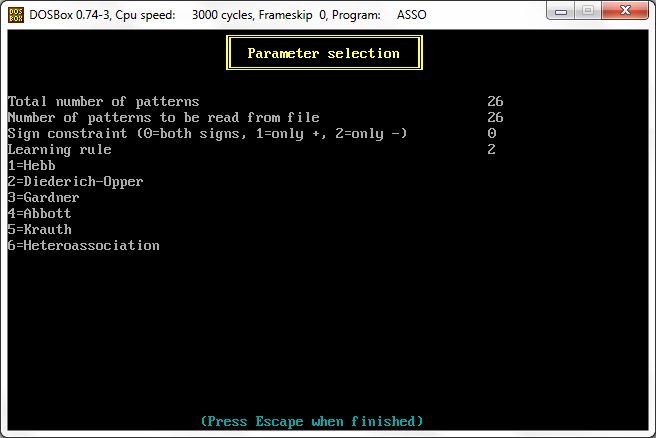
\includegraphics[scale=0.55]{ASSO_Capture_1}
\caption{Choice of the stored pattern and learning rule.}\label{ASSO_Capture_1}
\end{figure}
\begin{figure}[h!t]
\centering
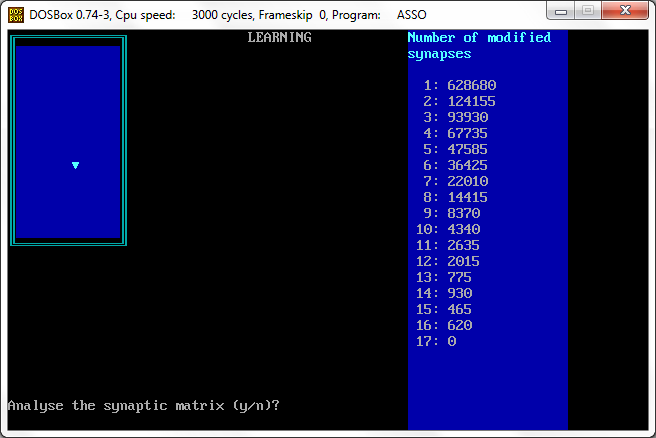
\includegraphics[scale=0.55]{ASSO_Capture_2}
\caption{Learning iterations.}\label{ASSO_Capture_2}
\end{figure}
\begin{figure}[h!t]
\centering
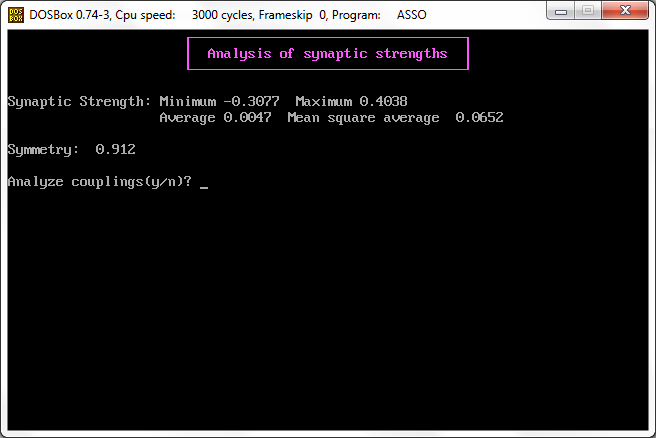
\includegraphics[scale=0.55]{ASSO_Capture_3}
\caption{Information on the synaptic strengths.}\label{ASSO_Capture_3}
\end{figure}
\begin{figure}[h!t]
\centering
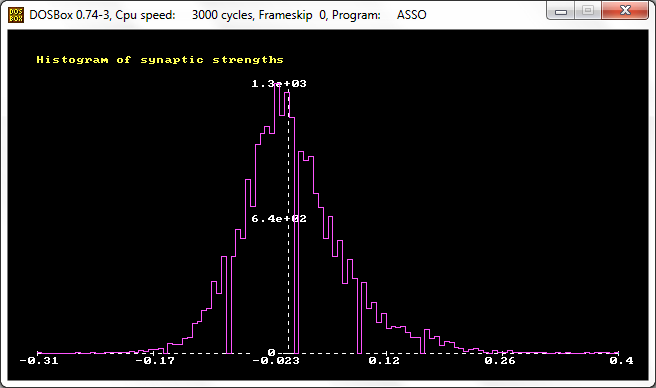
\includegraphics[scale=0.55]{ASSO_Capture_4}
\caption{Histogram of the synaptic strengths.}\label{ASSO_Capture_4}
\end{figure}
\begin{figure}[h!t]
\centering
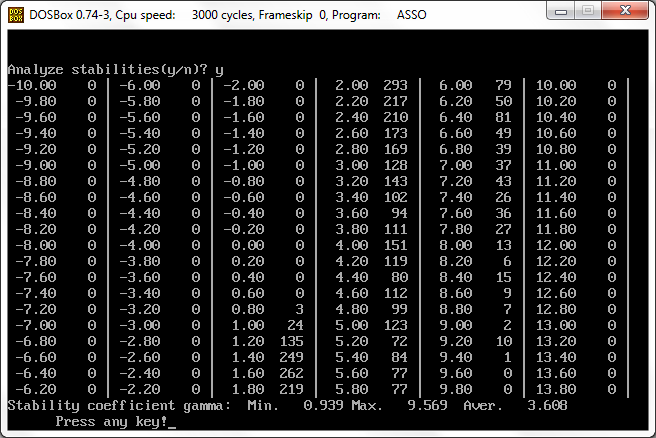
\includegraphics[scale=0.55]{ASSO_Capture_5}
\caption{Stability coefficients.}\label{ASSO_Capture_5}
\end{figure}
\begin{figure}[h!t]
\centering
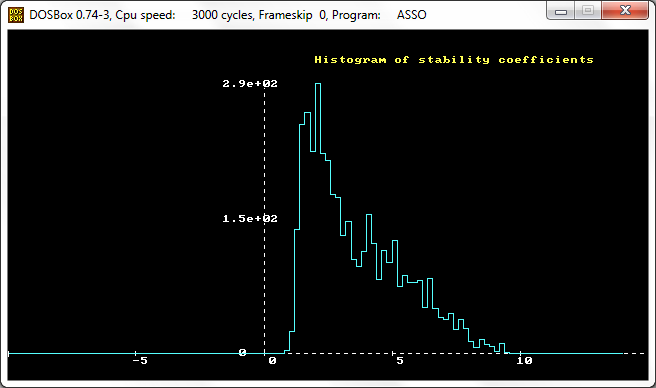
\includegraphics[scale=0.55]{ASSO_Capture_6}
\caption{Histogram of the stability coefficients.}\label{ASSO_Capture_6}
\end{figure}
\begin{figure}[h!t]
\centering
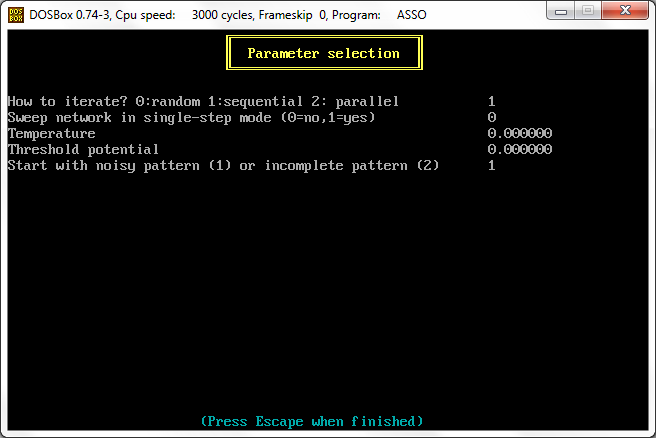
\includegraphics[scale=0.55]{ASSO_Capture_7}
\caption{Testing the neural network: choice of the parameters.}\label{ASSO_Capture_7}
\end{figure}
\begin{figure}[h!t]
\centering
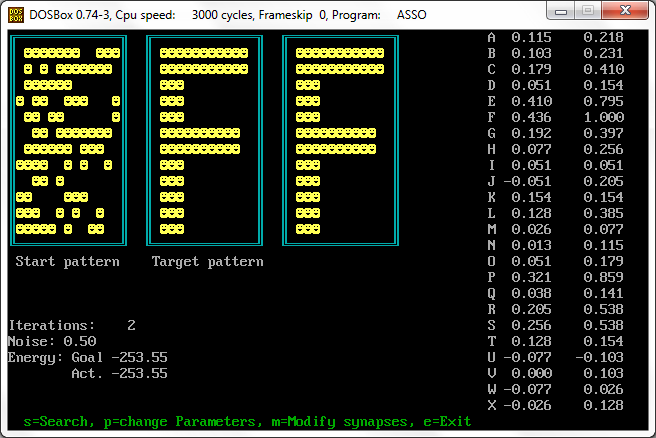
\includegraphics[scale=0.55]{ASSO_Capture_8}
\caption{Results of the execution.}\label{ASSO_Capture_8}
\end{figure}
\clearpage

\section[ASSCOUNT: associative memory for time sequences]{\textattachfile[color=0 0 0,modified=20210414124406+01'00',size=57393]{Attachments/ASSCOUNT.rar}{ASSCOUNT}: associative memory for time sequences}\label{sec:ASSCOUNT}
An obvious way to teach a Hopfield-type network to reproduce time sequences instead of stationary patterns is to introduce synaptic coefficients with an intrinsic time dependence as discussed in Sec.~\ref{sec:Neuralmotionpictures}. Thus instead of the synaptic matrix $w_{ij}$, which acts instantaneously to generate the local field defined in \eqref{ASSOfield}, one may introduce a collection of synapses $w_{ij}^\tau$ acting with a distribution of characteristic time delays of magnitude $\tau$. The local field, which according to \eqref{ASSOdeterministic} determines the probability for the updated neuron state $s_i(t+1)$, can be replaced by a generalized convolution in time.
\begin{equation}\label{ASSCOUNTfield}
h_i(t)=\sum_{\tau=0}^{\tau_{\text{max}}}\sum_{j=1}^N\lambda^\tau w_{ij}^\tau s_j(t-\tau)
\end{equation}
Here the coefficients $\lambda^\tau$ determine the relative strength of the various types of synaptic couplings. The ordinary Hopfield model corresponds to the case $\lambda^0=1$, $\lambda^\tau=0$ for $\tau\geq1$. The couplings in \eqref{ASSCOUNTfield} can give rise to a complex time evolution of the network. In the simplest nontrivial case just two types of synapse are present. We study a network connected through prompt synapses $w_{ij}$ and slow synapses $w_{ij}'$ of relative strength $\lambda$ with the fixed time delay $\tau$. The local field reads (cf. Sec.~\ref{sec:Neuralmotionpictures})
\begin{equation}
h_i(t)=\sum_{j=1}^Nw_{ij}s_j(t)+\lambda\sum_{j=1}^Nw_{ij}'s_j(t-\tau)
\end{equation}
Such a network can be made to go through an ordered sequence of patterns $1\rightarrow2\rightarrow3\rightarrow\ldots$ To this end the couplings $w_{ij}'$ have to provoke the transition between successive patterns in the series. This is achieved by a very simple modification of the learning rules. For example, the Hebb rule \eqref{ASSOHebb} for heteroassociation of the pattern $\sigma^{\mu+1}$ given the pattern $\sigma^\mu$ as an input reads
\begin{equation}
w_{ij}'=\frac{1}{N}\sum_{\mu=1}^p\sigma_i^{\mu+1}\sigma_j^\mu
\end{equation}
The improved learning rules can be modified in the same way by replacing $\sigma_i^\mu$ by $\sigma_i^{\mu+1}$ in the updating rule for $\delta w_{ij}^\mu$. The instantaneous synapses $w_{ij}$ are used to stabilize the patterns; thus they are trained in the ordinary way for the task of autoassociation. If the coefficient $\lambda$ is large enough, the network will act as a freely running counter. The state of the network will switch from
one pattern to the next after $\tau$ clock ticks when the delayed coupling starts to `pull in the direction' of the new pattern.

A second interesting mode of operation of this network arises if the parameter $\lambda$ is a little too small to induce transitions by itself. Then it takes an external disturbance to destabilize the old pattern. Once the network is driven out of the basin of attraction of the last pattern into some unstable region the delayed coupling $w_{ij}'$ (which does not yet feel the disturbance) provides a driving force toward the associated next pattern. Thus the network performs the task of counting the number of externally entered signal pulses. Such a pulse can be implemented by adding a spike of random noise with amplitude $\rho$ to the local field
\begin{equation}\label{ASSCOUNTrho}
h_i(t)=\sum_{j=1}^Nw_{ij}s_j(t)+\lambda\sum_{j=1}^Nw_{ij}'s_j(t-\tau)+\rho\xi_i\delta_{t,t_0}
\end{equation}
where $\xi_i$ is a random variable taking on values $\pm1$.
\subsection{Program description}
The program \texttt{ASSCOUNT.C} is closely related to \texttt{ASSO.C} so that much of the discussion of the last section applies here also. We assume that the reader is already familiar with \texttt{ASSO.C}. Again the total number of patterns \texttt{patts} and the number of predefined patterns \texttt{plett} to be learned must be specified. For a difference, the ordered patterns take the shape of the ten numerals $0,\ldots,9$ which are provided on the input file \texttt{ASSCOUNT.PAT}. The data format is the same as in the file \texttt{ASSO.PAT} so that by copying this file to the new name it is possible also to use the sequence of 26 letters instead of the numerals as patterns for counting.

Since our interest now is no longer focused on the learning process, only two choices are provided: Hebb's rule and the iterative scheme of Diederich and Opper. Learning takes about twice as much time since the synaptic matrices $w_{ij}$ and $w_{ij}'$ have to be learned separately. The learned association of patterns is cyclical, i.e. the last pattern in the series, $\sigma_i^p$, is followed again by $\sigma_i^1$.

After learning is finished you are asked to specify the following set of parameters:
\begin{itemize}
\item \texttt{update}: The rule of updating the network which can be random or sequential.
\item \texttt{sstep}: Single-step mode.
\item \texttt{temp}: The operating temperature $T$ of the network.
\item \texttt{tau}: The time delay of the couplings $w'$, an integer in the range $[1,10]$.
\item \texttt{lambda}: The relative strength of the delayed compared to the prompt couplings.
\item \texttt{rho}: The amplitude of the counting signal as defined in \eqref{ASSCOUNTrho}.
\end{itemize}

The iteration of the network is started by providing the starting pattern for which a pixel representation of one of the numbers $0,\ldots,9$ can be chosen (of course, if you have changed the input file \texttt{ASSCOUNT.PAT} the patterns may look very different). You can start with a distorted version of this pattern, specifying a value $\texttt{noise}\neq0$. The network is updated for \num{10000} sweeps unless the iteration is interrupted manually. As in \texttt{ASSO.C} the running parameters can be modified and the iteration restarted. The external signal for triggering the counter is entered by pressing \texttt{<SPACE>}.

To have the delayed network configuration $s_i(t-\tau)$ available at any instant $t$, all the intermediate values $s_i(t-1),\ldots,s_i(t-\tau)$ have to be stored. To avoid unnecessary data shuffling these values are stored in a cyclical buffer \texttt{s0[t][i]} of length \texttt{tau}. Two pointers \texttt{t\_in} and \texttt{t\_out} specify the locations where a configuration is stored and read out. These pointers are incremented after each sweep of the network using modulo $\tau$ arithmetic to account for the cyclical nature of the buffer.
\subsection{Numerical experiments}
You might start with the set of 10 numerals (which corresponds to a modest memory loading factor $\alpha=0.064$), using the learning rule for correlated patterns. At temperature $T=0$, experiment with the parameter $\lambda$. Essentially, different operating modes of the network can be observed in the three distinct regions. $\lambda>\lambda_2$: freely running counter; $\lambda_1<\lambda<\lambda_2$: counter for input signals. $\lambda<\lambda_1$ : stable associative network. However, the transition between these parameter regions is soft. For $\lambda>2$ the network evolves like a perfect clock, i.e. each counting step has a length equal to the synaptic delay time $\tau$, since a jump of the action of the second term in \eqref{ASSCOUNTrho} immediately induces a transition to the next pattern. When reducing the value of $\lambda$ the transition from one pattern to the next often needs several sweeps and the clock runs slow.

Figure~\ref{ASSCOUNTPattern} shows an example of the spontaneously counting network with a marginal value of $\lambda$. For $\tau=1$ the network has not enough time to settle at the attractors; it will operate with distorted and superimposed patterns. A further reduction of $\lambda$ will eventually cause the network to `get stuck' at one of the attractors with high stability (for our patterns the first of them happens to be the number `8'). At $\lambda=0.4$ all the patterns are stable against spontaneous transitions. Now we are in the region where the network can serve as a perfect counter for external signals provided that their amplitude $\rho$ is large enough. The theoretical expectation for the required amplitude is $\rho>1-\lambda$ which is very roughly confirmed by our numerical experiment. Finally, below $\lambda=0.2$ the strength of the delayed synapses is too small to induce the correct transition even for counting pulses of arbitrary strength.
\begin{figure}[h!t]
\centering
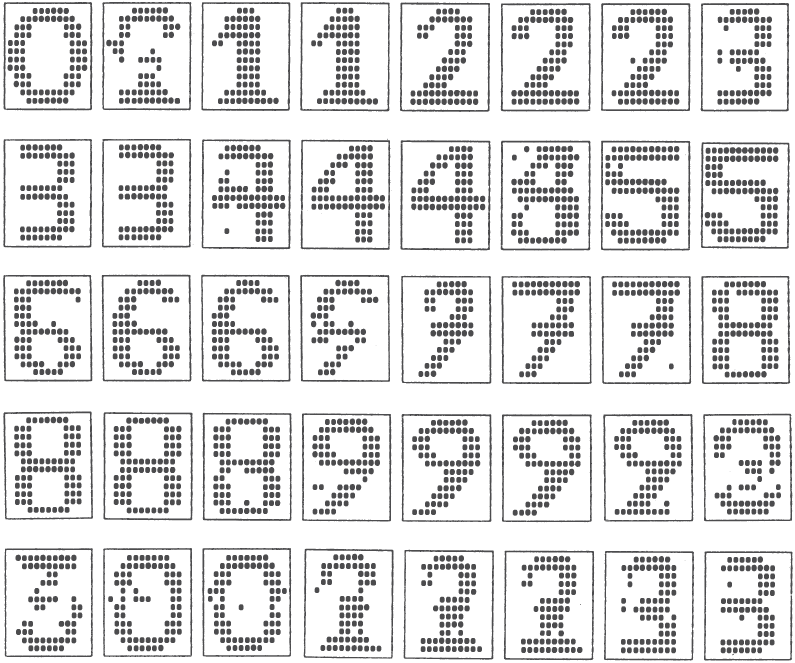
\includegraphics[scale=0.65]{ASSCOUNT Pattern}
\caption{The time development of a spontaneously counting network trained with the numeral patterns $0,\ldots,9$. The parameters are $\lambda=0.7$, $\tau=2$.}\label{ASSCOUNTPattern}
\end{figure}

The discussion so far referred to the fully deterministic case, $T=0$. Introducing a finite temperature has a profound influence on the network in the `chime counting' mode. Since the temperature-induced noise tends to destabilize a condensed pattern it aids the action of the delayed synapses. As soon as a sufficiently large fluctuation occurs, the state of the network will make a transition to the next pattern. E.g., take the parameters $\lambda=0.4$, $\tau=5$, which at zero temperature lead to a stationary network. At finite temperatures the network starts to count spontaneously! This effect can even serve as a `thermometer' since the cycle time is sensitive to the temperature (a rough estimate: $T=0.5$ gives a cycle length of 65; $T=0.15$ gives a cycle length of 120). Of course, at very high temperatures the network no longer reproduces any of the learned patterns while near $T=0$ the counting is frozen in long-lived metastable states.
\subsection{Snapshots}
\begin{figure}[h!t]
\centering
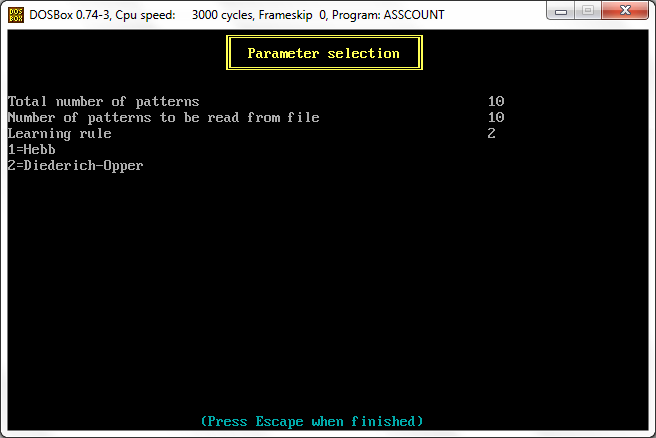
\includegraphics[scale=0.55]{ASSCOUNT_Capture_1}
\caption{Selection of patterns and learning rule.}\label{ASSCOUNT_Capture_1}
\end{figure}
\begin{figure}[h!t]
\centering
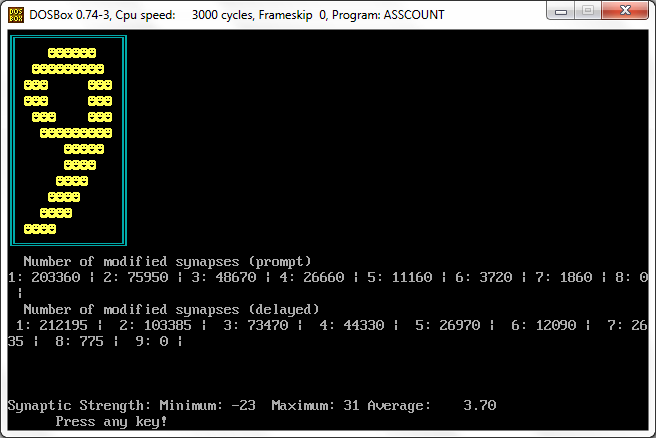
\includegraphics[scale=0.55]{ASSCOUNT_Capture_2}
\caption{Learning process.}\label{ASSCOUNT_Capture_2}
\end{figure}
\begin{figure}[h!t]
\centering
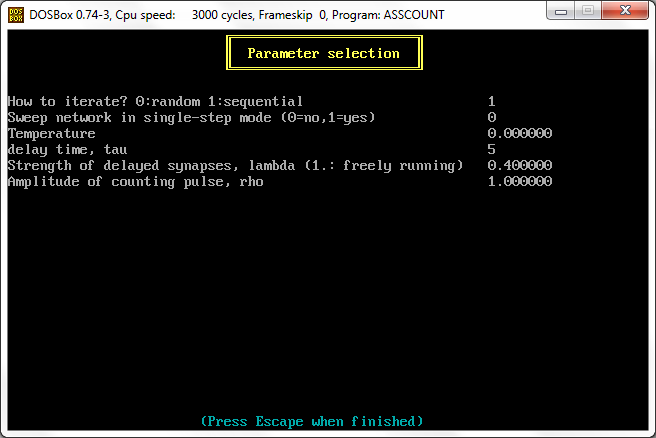
\includegraphics[scale=0.55]{ASSCOUNT_Capture_3}
\caption{Parameters selection.}\label{ASSCOUNT_Capture_3}
\end{figure}
\begin{figure}[h!t]
\centering
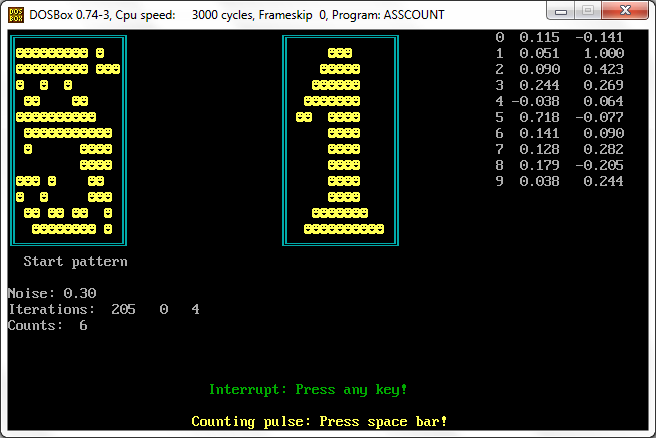
\includegraphics[scale=0.55]{ASSCOUNT_Capture_4}
\caption{Iteration of the network.}\label{ASSCOUNT_Capture_4}
\end{figure}
\clearpage

\section[PERBOOL: learning Boolean functions with back-propagation]{\textattachfile[color=0 0 0,modified=20210402125410+01'00',size=58189]{Attachments/PERBOOL.rar}{PERBOOL}: learning Boolean functions with back-propagation}\label{chap:PERBOOL}
This program illustrates the function of a feed-forward layered neural network as described in Sections~\ref{Sec:SimplePerceptron}--\ref{sec:Multilayerperceptron}. Its task is to learn an arbitrary Boolean function of a small number of Boolean variables. This is achieved by a three-layer feed-forward network which is trained by a gradient-descent method, i.e. by the rule of error back-propagation. The network consists of an input layer $\sigma_k$, $1\leq k\leq N_{\text{in}}$, a hidden layer $s_j$, $1\leq j\leq N_{\text{hid}}$, and an output layer $S_i$, $1\leq i\leq N_{\text{out}}$. The synaptic connections are $\overline{w}_{jk}$ from the input to the hidden layer, and $w_{ij}$ from the hidden to the output layer. In addition there are activation thresholds $\overline{\vartheta}_j$ and $\vartheta_i$. The neurons have two activation values chosen as $-1$ and $+1$ (the transformation to the values 0 and 1 commonly used to represent binary numbers is trivial).

When an input pattern is fed into the network by clamping the neurons $\sigma_k$ to represent an input pattern, the activation of the intermediate and output layers is determined according to the rule (\ref{eq:eqn922-1}--\ref{eq:eqn922-2}), namely
\begin{alignat}{2}
S_i&=f(h_i)\,, &\qquad\quad h_i&=\sum_{j=1}^{N_{\text{hid}}}w_{ij}s_j-\vartheta_i\\
s_j&=f\bigl(\overline{h}_j\bigr)\,, &\qquad\quad \overline{h}_j&=\sum_{k=1}^{N_{\text{in}}}\overline{w}_{jk}\sigma_k-\overline{\vartheta}_j
\end{alignat}
The activation function $f(x)$ for discrete two-state neurons corresponds to the step function $f(x)=\sgn{x}$. During the learning phase, however, this is replaced by the continuous ``sigmoidal'' function
\begin{equation}
f(x)=\tanh{(\beta x)}
\end{equation}
since gradient learning is possible only if $f(x)$ is a smooth function with a finite derivative, which in our case is $f'(x)=\beta\sech^2{(\beta x)}$. At the end of the training phase the limit $\beta\rightarrow\infty$ leading to a discontinuous activation function is taken. As said in Sec.~\ref{Sec:SimplePerceptron}, if one wishes to work with two-state neurons throughout the training process, one can simply replace the derivative function $f'(x)$ by an averaged constant, which can be absorbed in the factor $\varepsilon$ (see below).

The rule for error back-propagation minimizing the squared deviation of the network output from the target values according to (\ref{eq:deltaw}--\ref{eq:deltabarjmu}) leads to the synaptic corrections
\begin{alignat}{3}
\delta w_{ij}&=\varepsilon\sum_{\mu=1}^p\Delta_i^\mu s_j^\mu\,, &\qquad \delta\vartheta_i&=-\varepsilon\sum_{\mu=1}^p\Delta_i^\mu\,, &\qquad \Delta_i^\mu&=\Bigl[\zeta_i^\mu-f\bigl(h_i^\mu\bigr)\Bigr]f'\bigl(h_i^\mu\bigr)\label{PERBOOL:4.04}\\
\delta\overline{w}_{jk}&=\varepsilon\sum_{\mu=1}^p\overline{\Delta}_j^\mu\overline{s}_k^\mu\,, &\qquad \delta\overline{\vartheta}_j&=-\varepsilon\sum_{\mu=1}^p\overline{\Delta}_j^\mu\,, &\qquad \overline{\Delta}_j^\mu&=\left(\sum_{i=1}^{N_{\text{out}}}\Delta_i^\mu w_{ij}\right)f'\bigl(\overline{h}_j^\mu\bigr)
\end{alignat}
%The changes of the threshold values $\delta\vartheta_i,\delta\overline{\vartheta}_j}$ are determined by nearly identical formulae. These are obtained by simply replacing the input signal ($s_j^\mu$ or $\sigma_k^\mu$) by the fixed value -

A simple modification of the learning procedure consists in the replacement of \eqref{PERBOOL:4.04} by
\begin{equation}\label{PERBOOL:4.06}
\Delta_i^\mu=\beta\Bigl[\zeta_i^\mu-f\bigl(h_i^\mu\bigr)\Bigr]
\end{equation}
This change has the potential to speed up the convergence: the weight adjustments get increased in the ``saturation region'' where the value of $h_i^\mu$ is large and the factor $f'(h_i^\mu)$ approaches zero. For small values of $h_i^\mu$ \eqref{PERBOOL:4.06} agrees with \eqref{PERBOOL:4.04}.

The learning consists of consecutive ``training epochs'' in which the full set of patterns $\sigma_k^\mu$ to be learned is presented to the network. The synaptic and threshold corrections are accumulated and applied at the end of an epoch. As a variation of this ``batch learning'' algorithm one can also update the network parameters after each single presentation of a pattern. This `online learning' may, but is not guaranteed to, improve the learning speed.

An important modification which has the potential to improve the stability of the learning process consists in the introduction of a kind of hysteresis effect or ``momentum''. In regions of the parameter space where the error surface is strongly curved the gradient terms $\Delta$ can become very large. Unless the parameter $\varepsilon$ is chosen to be inordinately small, the synaptic corrections $\delta w_{ij}$ will then tend to overshoot the true position of the minimum. This will lead to oscillations which can slow down or even foil the convergence of the
algorithm. To avoid this problem the correction term can be given a memory in such a way that it will no longer be subject to abrupt changes. This is achieved by the prescription
\begin{equation}
\delta w_{ij}^{(n)}=\varepsilon\sum_{\mu=1}^p\Delta_i^\mu s_j^\mu+\alpha\delta w_{ij}^{(n-1)}
\end{equation}
where the index $n$ denotes the number of the training epoch. In the language of numerical analysis this is called a \emph{relaxation} procedure. If $\alpha$ is chosen fairly large, the search in the parameter space will be determined by the gradient accumulated over several epochs, which has a stabilizing effect. Unfortunately there is no general criterion how the gradient parameter $\varepsilon$ and the momentum parameter $\alpha$ are to be chosen. The optimal values depend on the problem to be learned.
\subsection{Program description}\label{sec:C.1}
The progam \texttt{PERBOOL.C} implements a three-layer network with dimensions $\texttt{nin}\leq5$, $\texttt{nhid}\leq100$, $\texttt{nout}\leq5$. The desired values can be entered through an input panel which comes up immediately after starting the program.

The \texttt{nin} Boolean input variables can take on $\texttt{nbin}=2^{\texttt{nin}}$ different values. The network is trained with a set of $\texttt{patts}=\texttt{nbin}$ output patterns, i.e. the output is completely prescribed for each possible input combination\footnote{To study the issue of generalization one would train the network with a subset of all possible inputs, i.e. use a smaller value of \texttt{patts}.}. Even in the ``scalar'' case, i.e. for a single output variable, $\texttt{nout}=1$, there is an embarrassing number of $2^{2^{\texttt{nin}}}$ possible Boolean functions. To define an arbitrary Boolean function we have to select a set of \texttt{nout} bit strings having the length \texttt{nin}.
%$2^{\texttt{nin}}$. or because hexadecimal?

These bit strings are represented in the program by the long integer variables \texttt{key[i]}, which conveniently can hold just 32 bits. Each bit specifies the desired response of the corresponding output neuron to that combination of input values which is encoded by the binary value of the position of the bit within the variable key. Since this may sound confusing, let us look at the familiar example of the \textsc{xor} function. There are $2^2=4$ combinations of the two input variables and the output is defined by $00\rightarrow0$, $01\rightarrow1$, $10\rightarrow1$, $11\rightarrow0$. The input can be interpreted as a 2-bit binary number. Stepping through its value in descending order, the output is represented by the bit string 0110. Thus the \textsc{xor} function is encoded by specifying the number $\texttt{key}={0110}_{\text{bin}}={6}_{\text{hex}}={6}_{\text{dec}}$.

The Boolean function to be learned can be defined for the program by giving the code number(s) \texttt{key[i]} for $\texttt{i}=1,\ldots,\texttt{nout}$ in hexadecimal representation, with the digits 0123456789ABCDEF. Since in general it is somewhat tedious to work out this binary code, the program allows for an alternative and more direct way of specifying the Boolean function. Having answered `\texttt{m}' to the prompt, a menu is displayed in which the desired output bits can be directly entered by moving the cursor to the appropriate place, typing 0 or 1, and pressing \texttt{<Return>}. Note that for the case $\texttt{nout}>1$ the complete output string $\zeta_i^\mu$, $\texttt{i}=1,\ldots,\texttt{nout}$, has to be entered: it is not possible to modify single bits. The program displays the hexadecimal value of the resulting coding variable(s) key which will facilitate the data entry if the same function is to be used repeatedly. The decoding of the input and output patterns takes place in the subroutine \texttt{patterns()} and produces the arrays $\texttt{zetp}=\zeta_i^\mu$ and $\texttt{sigp}=\sigma_k^\mu$.

Having been given the Boolean function to be learned, the program displays a second input panel which allows to specify details of the learning procedure.
\begin{itemize}
\item \texttt{epsilon}: The learning rate $\varepsilon$.
\item \texttt{alpha}: The ``momentum'' constant $\alpha$.
\item \texttt{batch}: Selects the learning protocol ($\texttt{online}=0$, $\texttt{batch}=1$) .
\item \texttt{mod\_cost}: Use of the modified cost function (see equation \eqref{PERBOOL:4.06}).
\item \texttt{beta}: The inverse steepness $\beta$ of the activation function $f(x)$.
\end{itemize}

Subsequently the program enters the subroutine \texttt{learn()}. The synaptic coefficients and thresholds are initialized with random numbers in the range $-1<\xi<+1$. Then one by one the input patterns are presented and a forward sweep is performed leading to output activations \texttt{sout[i]}. The difference of these values from the correct output \texttt{zout[i]} allows the calculation of modified network parameters according to the back-propagation algorithm. After each learning epoch the accumulated error $\sum_\mu\sum_i\bigl\lvert\zeta_i^\mu-S_i^\mu\bigr\rvert$ is shown. In addition the actual values of the network parameters are displayed on screen. Each line in the display shows the connections attached to one of the hidden neurons according to the following format:

{\centering
\begin{table}[h!t]
\centering
\newcolumntype{C}{>{$}c<{$}}
\renewcommand{\arraystretch}{1.25}
\begin{tabular}{CCC|C|CCC}
\hline
\overline{w}_{1,1}	& \cdots	& \overline{w}_{1,\texttt{nin}}	& \overline{\vartheta}_1	& w_{1,1}	& \cdots	& w_{\texttt{out},1}\\
\vdots	& \ddots	& \vdots	& \vdots	& \vdots	& \ddots	& \vdots \\
\overline{w}_{\texttt{nhid},1}	& \cdots	& \overline{w}_{\texttt{nhid},\texttt{nin}}	& \overline{\vartheta}_{\texttt{nhid}}	& w_{1,\texttt{nhid}}	& \cdots	& w_{\texttt{out},\texttt{nhid}}\\
\hline
\multicolumn{4}{c|}{}	& \vartheta_1	& \cdots	& \vartheta_{\texttt{nout}}
\end{tabular}
\caption{Format used for output of network configuration.}\label{PERBOOL:tab}
\end{table}
}

If the number of hidden neurons is large, only the first 20 lines of this table are displayed in order not to overflow the screen.

After any learning epoch the user can interrupt the learning by pressing the key `\texttt{r}'. This serves to evaluate the network performance using the current coupling coefficients. Displayed are the states of the input, intermediate, and output neurons, with a flagging of the wrong output bits. Note that this display employs the discrete activation function, so that the number of wrong bits may deviate from that contained in the error variable.

By pressing `\texttt{p}' it is possible to view and modify the values of the parameters used by the back-propagation algorithm during the learning process.

Perhaps more illuminating---and at least more entertaining---than the numerical output is a graphical representation of the learning process. This mode is entered if the key `\texttt{g}' is pressed during learning. Then as a function of the learning epoch a collection of $\texttt{patts}=2^{\texttt{nin}}$ curves is shown. Each curve represents the activation of the (first) output neuron in response to one specific input pattern. Since in the learning phase the network operates with continuous functions $f(x)$, these curves move smoothly in the interval $[-1,+1]$. The abscissa extends over a range of 200 training epochs. If this number is exceeded, the display is erased and the curves reappear at the left border. By repeatedly pressing `\texttt{g}' one can switch between graphics and text
display.

If the learning converges to the correct solution, the program tries to make a smooth transition to the discrete (i.e. theta-function) operating mode by slowly increasing the value of $\beta$ by a factor of $1.05$ after each epoch. This sets in if the error variable falls below the value $1/\beta$ and continues until error reaches $10^{-3}$.

After convergence has been reached or when the learning process is stopped by pressing the key `\texttt{e}' the complete set of synaptic coefficients and thresholds is displayed and the final network performance is shown.

We should mention that initially the program operates in the `slow motion' mode, inserting a delay of $0.5$ second in each training epoch. By pressing the key \texttt{s} it is possible to switch to full speed.
\subsection{Numerical experiments}
The simplest example of a Boolean function with a nontrivial representation is the exclusive-\textsc{or} problem (\textsc{xor}) discussed in Sec.~\ref{sec:Theexclusivexor}. This can be investigated by setting $\texttt{nin}=2$, $\texttt{nout}=1$, and $\texttt{key}=6$. The back-propagation algorithm can solve this problem without much effort provided that the network configuration contains at least two hidden units, $\texttt{nhid}=2$. Over a fairly wide range of parameters $\varepsilon$ and $\alpha$ most learning runs lead to convergence to a valid solution. One typically might choose a gradient parameter $\varepsilon=1$ and a momentum factor $\alpha=0.9$. The steepness parameter $\beta$ in principle is redundant and may be kept fixed at the value $\beta=1$. Owing to the special form of the activation function $f(x)$, this parameter only enters as a multiplicative factor attached to the local fields $h_i$. Therefore a change of $\beta$ can be offset by inversely rescaling all synaptic coefficients and thresholds. If also the gradient parameter $\varepsilon$ is rescaled (quadratically), the behavior of the network should be unchanged. In our program implementation this is not quite true since the initialization is performed with random numbers in the fixed interval $-1<\xi<1$. If a very small value of $\beta$ is chosen, this has the same effect as an initialization with near-zero values, which adversely affects the convergence behavior.

Examining the performance of the network, one can notice that it finds a considerable variety of solutions to the \textsc{xor} problem. Most solutions are essentially equivalent, differing by simultaneous sign changes of activation values $s$ and coupling coefficients $w$ which leave invariant the equations which describe the network. This is a reflection of the fact that with the help of negation operations the \textsc{xor} function can be represented in various ways by using the de Morgan identity of Boolean algebra $\overline{A\land B}=\overline{A}\lor\overline{B}$. There are two distinct classes of representation of \textsc{xor} where the output neuron acts either as an \textsc{or} gate or as an \textsc{and} gate, according to
\begin{gather}
A\oplus B=(A\lor B)\land\overline{A\land B}\label{XORrepr1}\\
A\oplus B=(A\land\overline{B})\lor(\overline{A}\land B)\label{XORrepr2}
\end{gather}
where $\oplus$ is used to denote the exclusive-\textsc{or} or \textsc{or} function. An example of the former solution type was shown in Fig.~\ref{img:MultilayeredXOR}. The following two tables show typical results of couplings and thresholds generated by the back-propagation algorithm. They are displayed in the format introduced in the last subsection
\begin{table}[h!t]
\centering
\newcolumntype{C}{ >{$}c<{$} }%S[table-format=-1.3]
\renewcommand{\arraystretch}{1.15}
\begin{subtable}[ht]{0.495\textwidth}
	\centering
	\begin{tabular}{CC|C|C}
	\hline
	+1.657 & +1.615 & -1.968 & +3.105 \\
	+2.536 & +2.929 & +3.155 & -2.494 \\
	\hline
	\multicolumn{3}{c|}{} & +2.306 \\
	\end{tabular}
	\caption{Example of \eqref{XORrepr1}.}\label{PERBOOL:tab2.1}
\end{subtable}
%\hfill
\begin{subtable}[ht]{0.495\textwidth}
	\centering
	\begin{tabular}{CC|C|C}
	\hline
	+2.059 & -2.034 & +2.368 & +3.117 \\
	-2.432 & +2.624 & +2.518 & +2.623 \\
	\hline
	\multicolumn{3}{c|}{} & -2.153 \\
	\end{tabular}
	\caption{Example of \eqref{XORrepr2}.}\label{PERBOOL:tab2.2}
\end{subtable}
\caption{}\label{PERBOOL:tab2}
\end{table}

Starting from randomly initialized couplings, the learning algorithm often converges within about 20 iteration steps. However, it does not always find valid solutions of the \textsc{xor} problem. In some instances it gets stuck at a local minimum, or the local fields are driven to large values where the derivative of the activation function $f'(h)$ is nearly zero, leading to exceedingly slow learning. Figure~\ref{PERBOOLLearningGraph} shows an example where the network has just managed to escape from such a situation after about 100 training epochs.
\begin{figure}[h!t]
\centering
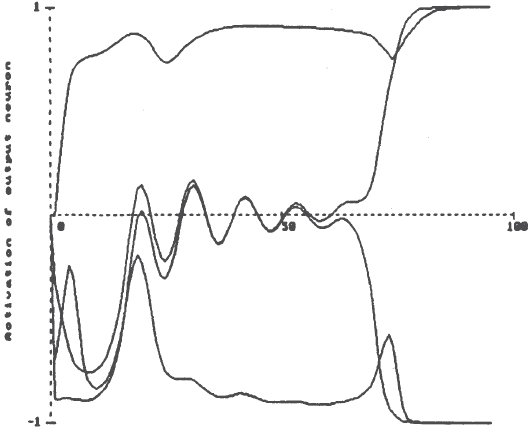
\includegraphics[scale=0.6]{PERBOOL Learning Graph}
\caption{A 2--2--1 perceptron learns the function \textsc{xor}. The curves depict the activation of the output
neuron $S$ when the network is presented with the four possible input patterns as a function of training epochs. Parameters: $\varepsilon=0.1$, $\alpha=0.9$, $\beta=1$.}\label{PERBOOLLearningGraph}
\end{figure}

Going to problems of a higher dimension provides further insights. As the `benchmark' problem we have predefined in the program PERBOOL the generalization of the \textsc{xor} function to more than two variables. This function takes on the value 1 if there is an odd and 0 if there is an even number of 1s in the input. Thus it can also be called the `parity' function; still another interpretation is `addition modulo 2'. Let us take the case $\texttt{nin}=5$. Using the binary encoding of the Boolean function leads to $\texttt{key}={10010110011010010110100110010110}_{\text{bin}}={96696996}_{\text{hex}}$. The parity problem can be learned if the number of hidden neurons is at least equal to the input dimension, $\texttt{nhid}=\texttt{nin}$. However, even for $\texttt{nhid}=\texttt{nin}-1$ the network can produce solutions while operating with continuous activation functions. It is not too surprising that continuous variables $s_i$ can encode more information than discrete ones. This solution is destroyed in the final stage of the learning process when the program tries to perform the limit $\beta\rightarrow\infty$.

Other interesting examples with $\texttt{nin}=5$ the reader might wish to study are the mirror symmetry function ($\texttt{key}={88224411}_{\text{hex}}$) and the shift register ($\texttt{key}_1=\text{AAAAAAAA}_{\text{hex}}$, $\texttt{key}_2=\text{FFFF0000}_{\text{hex}}$, $\texttt{key}_3=\text{FF00FF00}_{\text{hex}}$, $\texttt{key}_4=\text{F0F0F0F0}_{\text{hex}}$, $\texttt{key}_5=\text{CCCCCCCC}_{\text{hex}}$).

The \emph{symmetry function} signals whether the input bit pattern has mirror symmetry. As an example the following table shows the weights and thresholds of a 5--2--1 network which can recognize this property\footnote{Incidentally, two hidden neurons are sufficient to solve the mirror-symmetry problem of arbitrary dimension!}.
\begin{table}[h!t]
\centering
\newcolumntype{C}{>{$}c<{$}}
\renewcommand{\arraystretch}{1.25}
\begin{tabular}{CCCCC|C|C}
\hline
+2.248 & -1.058 & +0.029 & +1.020 & -2.196 & -1.149 & +3.113 \\
-2.659 & +1.289 & +0.021 & -1.284 & +2.628 & -1.066 & +2.759 \\
\hline
\multicolumn{6}{c|}{} & +2.627 \\
\end{tabular}
\caption{}\label{PERBOOL:tab3}
\end{table}

We note the antisymmetric structure of the couplings in the input layer. The mirror symmetry property of a 5-bit pattern does not depend on the bit in the center. We observe that the third input unit is indeed decoupled and has no influence on the state of the network. The output layer performs a logical conjunction of the states of the two hidden neurons. The solution found above was obtained using the parameters $\varepsilon=0.01$, $\alpha=0.9$, $\beta=1$. However, very often the back-propagation algorithm does not converge to a valid solution.
\subsection{Snapshots}
\begin{figure}[h!t]
\centering
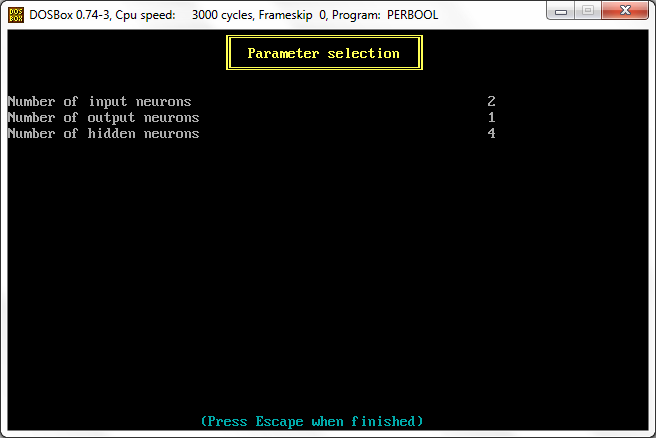
\includegraphics[scale=0.55]{PERBOOL_Capture_1}
\caption{Length of the input, hidden and output layers.}\label{PERBOOL_Capture_1}
\end{figure}
\begin{figure}[h!t]
\centering
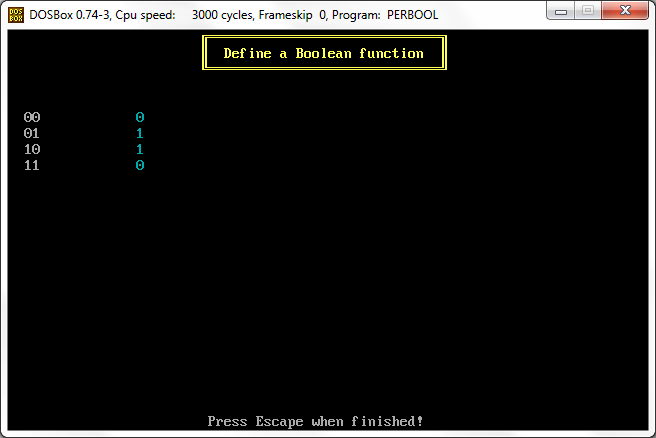
\includegraphics[scale=0.55]{PERBOOL_Capture_2}
\caption{Definition of the \textsc{xor} through its truth table.}\label{PERBOOL_Capture_2}
\end{figure}
\begin{figure}[h!t]
\centering
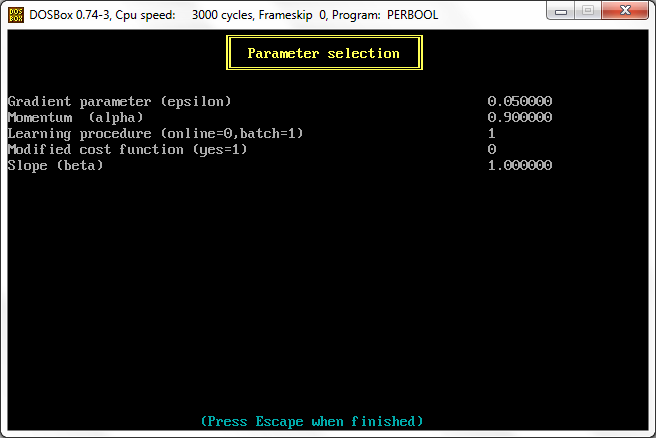
\includegraphics[scale=0.55]{PERBOOL_Capture_3}
\caption{Parameters of the learning protocol.}\label{PERBOOL_Capture_3}
\end{figure}
\begin{figure}[h!t]
\centering
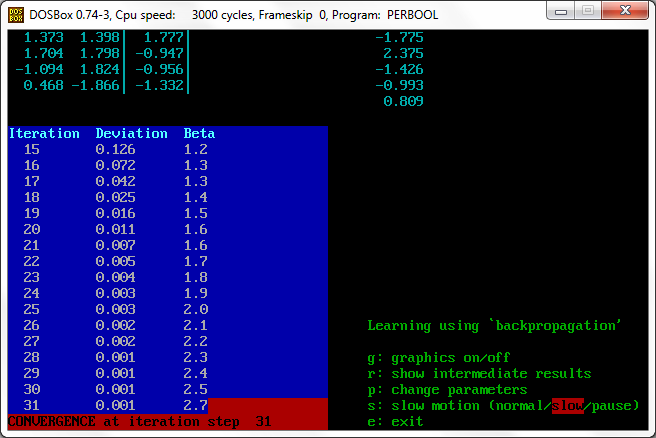
\includegraphics[scale=0.55]{PERBOOL_Capture_4}
\caption{Display of the training iterations.}\label{PERBOOL_Capture_4}
\end{figure}
\begin{figure}[h!t]
\centering
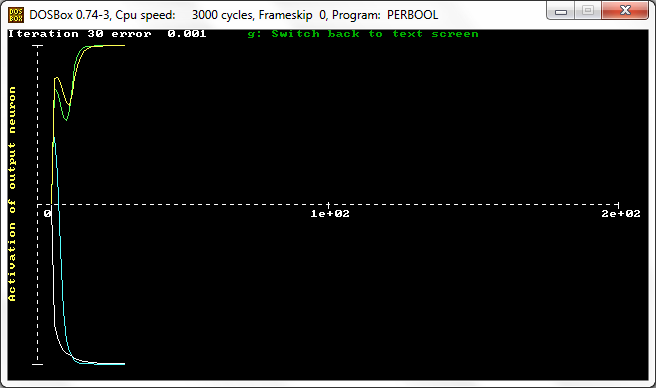
\includegraphics[scale=0.55]{PERBOOL_Capture_5}
\caption{Graphic representation of the learning process.}\label{PERBOOL_Capture_5}
\end{figure}
\begin{figure}[h!t]
\centering
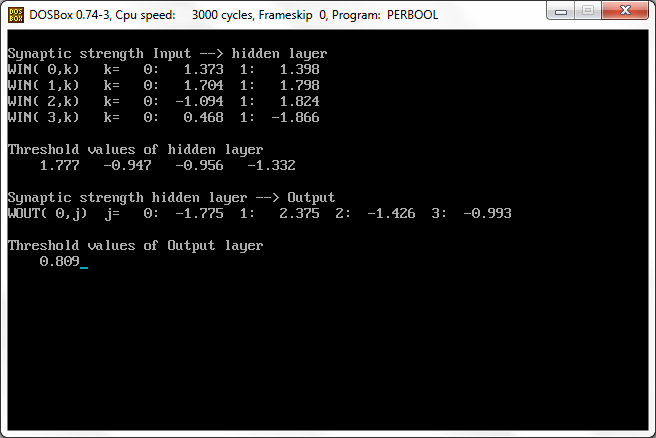
\includegraphics[scale=0.55]{PERBOOL_Capture_6}
\caption{Optimal synaptic coefficients and thresholds.}\label{PERBOOL_Capture_6}
\end{figure}
\begin{figure}[h!t]
\centering
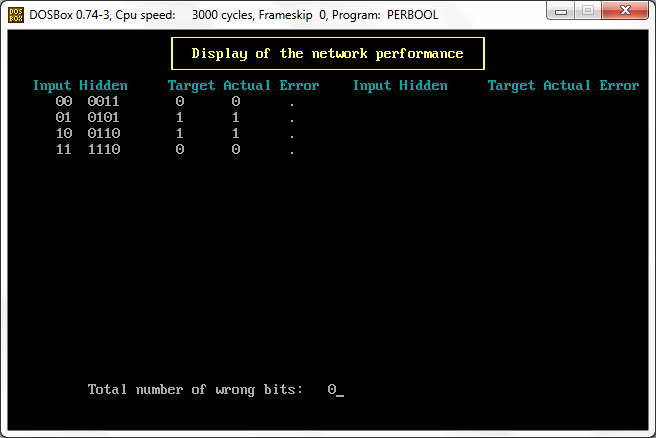
\includegraphics[scale=0.55]{PERBOOL_Capture_7}
\caption{Network performance.}\label{PERBOOL_Capture_7}
\end{figure}
\clearpage

\section[PERFUNC: learning continuous functions with back-propagation]{\textattachfile[color=0 0 0,modified=20210402125410+01'00',size=58189]{Attachments/PERFUNC.rar}{PERFUNC}: learning continuous functions with back-propagation}
As discussed in Sec.~\ref{sec:Continuousfunctions}, feed-forward networks with hidden layers can represent any smooth continuous function $\mathbb{R}^n\rightarrow\mathbb{R}^m$. As an illustration the program PERFUNC is designed to solve the following task: when presented with the values of a specimen $g(x)$ out of a class of one-dimensional functions at a set of points $x_i$, it predicts the function values at the output points $x_i'$. This is achieved by training the network with the error back-propagation algorithm by presenting various `patterns' $\sigma_i^\mu$ where $\mu$ refers to specific values of the continuous parameters on which the function $g(x)$ depends. The training method is essentially the same as was used for Boolean-function learning, so that its description need not be repeated. As a slight variation, the couplings $w_{ij}$ to the output layer are realized by \emph{linear} transfer functions $\tilde{f}(x)=x$. In contrast to the bounded sigmoidal function $f(x)=\tanh{(\beta x)}$ used for the interior layers, this enables the output signals $S_i$ to take on arbitrarily large values.
\subsection{Program description}
PERFUNC is closely related to the program PERBOOL described in Section~\ref{chap:PERBOOL}. Differences arise from the fact that \emph{0, 1, or 2 hidden layers} are allowed and from the way training patterns are provided. Since learning can take a long time, the synaptic coefficients and thresholds can be read in from a data file to provide for a fast demonstration of the network's capabilities. Alternatively, to operate in learning mode the following parameters can be specified via the input panel of the program.
\begin{itemize}
\item \texttt{nlayers}: The number of hidden layers which may take the values 0, 1, or 2.
\item \texttt{nin}, \texttt{nout}, \texttt{nhid}: The number of neurons in the input, output, and hidden layer. If there are two hidden layers, these will have equal numbers of neurons.
\item \texttt{ntyp}: The type of function $g(x)$ to be learned. The three choices are:
	\begin{itemize}
	\item $\displaystyle g_1(x)=c_1x+c_2$
	\item $\displaystyle g_2(x)=\sin{\left[\left(c_1x+\frac{1}{2}c_2\right)2\pi\right]}$
	\item $\displaystyle g_3(x)=c_2x^{1+c_1}$
	\end{itemize}
\item \texttt{nparm}: The number of function parameters, e.g. the frequency and phase of the sine function $g_2(x)$. If $\texttt{nparm}=1$, the second parameter is absent, $c_2=0$, or $c_2=1$ in the case of $g_3(x)$.
\item \texttt{patts}: The number of different patterns to be used in training. A pattern consists of the input and output values $\sigma_l$, $l=1,\ldots,\texttt{nin}$, $S_i$, $i=1,\ldots,\texttt{nout}$ produced by a representative of the class of functions $g(x)$. It is generated by randomly selecting values for the parameters $c_1$ and $c_2$ in the range $[-1,+1]$.
%S_i o \zeta_i?
\item \texttt{errmax}: Target value for the mean error per output neuron. Learning is stopped when this accuracy is reached.
\end{itemize}
Subsequently the program asks for the set of input and output coordinates $x_i$ and $x_i'$.

A second input panel asks for the following parameters which determine the learning phase:
\begin{itemize}
\item \texttt{epsilon}: The learning rate $\varepsilon$.
\item \texttt{alpha}: The ``momentum'' constant $\alpha$.
\item \texttt{multi}: The multiplicity of pattern presentations. If $\texttt{multi}>1$, the same pattern is presented repeatedly to the back-propagation algorithm before going to the next pattern (note: the momentum parameter $\alpha$ has no effect in this mode).
\item \texttt{fixpat}: This variable determines whether a fixed set of patterns is used for training, or whether at the beginning of each training epoch new patterns are chosen.
\item \texttt{beta}: The inverse steepness $\beta$ of the activation function $f(x)$.
\end{itemize}

The learning process is started by initializing all couplings and thresholds to random numbers in the range $[-1,1]$. After each learning epoch the current coupling and threshold values are displayed according to the format introduced in Sec.~\ref{sec:C.1}. For $\texttt{nlayers}=2$ only the parameters of the first hidden layer and the output layers are displayed; for $\texttt{nlayers}=1$ the lines (columns) correspond to the input (output) units of the network. In addition a listing of the error value as a function of the training epoch number is maintained. During the training phase the user can interact with the program in various ways. After pressing the key `\texttt{p}' the parameters which influence the learning process may be changed: \texttt{epsilon}, \texttt{alpha}, \texttt{multi}, \texttt{fixpat}, \texttt{beta}. With the key `\texttt{r}' the current network performance may be investigated. Finally, by pressing `\texttt{e}' the learning is stopped.

Three different choices are offered for examining the current performance:
\begin{itemize}
\item \texttt{n}: A numerical listing of the errors for an equidistant mesh of parameter values $c_1$, $c_2$ in the interval $[-1,1]$. If $\texttt{nparm}=1$, the values $S_1^{\mu=1}$, $\zeta_1^\mu$, and the mean square error $D^\mu=\sqrt{\sum_{i=1}^{\texttt{nout}}{\bigl(S_i^\mu-\zeta_i^\mu\bigr)}^2}$ are listed. For $\texttt{nparm}=2$ a table of values of $D^\mu$ is displayed, where the columns correspond to the variation of the second parameter $c_2$ with an increment of $0.2$, while the rows are calculated for different values of $c_1$ (increment $0.1$). In addition the mean error for all patterns is printed.
\item \texttt{p}: With this option the program shows a graphical plot of the deviations $S_i^\mu-\zeta_i^\mu$, $i=1,\ldots,\texttt{nout}$ as a function of the parameter $c_1$. The range of display and the value of $c_2$, which is kept fixed, can be entered.
\item \texttt{f}: The program prompts for the entry of the constants $c_1$ and $c_2$. Then a plot of the function $g(x)$ is drawn together with the input values $g(x_i)$ (marked by \texttt{+} symbols) and the output values $g(x_i')$ produced by the network (marked by \texttt{x}).
\end{itemize}

After a final examination of the network performance the couplings can be stored on a data file.
\subsection{Numerical experiments}
Since the learning of continuous functions is rather time consuming, it might be wise to start with very simple examples. There is only one case where an exact solution is possible: the linear network trained to represent a linear function. Indeed, for a 1--1 network trained with the general linear function $g_1(x)$ ($\texttt{nlayers}=0$, $\texttt{nin}=2$, $\texttt{nout}=1$, $\texttt{nparm}=1$) the learning algorithm quickly finds the solution, which is $w_{11}=\frac{x_2-x'}{x_2-x_1}$, $w_{12}=\frac{x'-x_1}{x_2-x_1}$, $\vartheta_1=0$. This is quite insensitive to the details of the training rule as long as the gradient parameter \texttt{epsilon} is not too large. Otherwise the algorithm becomes unstable and the weights `explode' , leading to an exponentially growing error. Learning is achieved both with a fixed set of `patterns' (i.e. combinations of $c_1$ and $c_2$) and with patterns which are selected at random in each step, although in the latter case the convergence is markedly slower. If there are more input values than necessary, the problem is underdetermined. This does not impede the learning process, but different sets of weights $w_{1i}$ are found in each run, because of the random initial conditions.

For a network with a \emph{nonlinear} transfer function $f(x)$ the representation of a linear function will not be exact. For the trivial 1--1--1 architecture ($\texttt{nlayers}=1$, $\texttt{nin}=1$, $\texttt{nhid}=1$, $\texttt{nout}=1$) trained with the one-parameter linear function the network represents the general function $S=w\tanh{(\overline{w}\sigma-\overline{\vartheta})}-\vartheta$. This has to provide a fit to the function $\zeta=(x'/x)\sigma\equiv c\sigma$. In principle this can be accomplished with arbitrary precision by scaling the weights so that the linear region of the $\tanh$ function is probed: $\overline{\vartheta}=\vartheta=0$, $\overline{w}=\varepsilon$, $w=c/\varepsilon$ with $\varepsilon\rightarrow0$. Experiments with the program show that a fairly good representation of the linear function can be achieved, but the relative size of the weights $w$ and $\overline{w}$ remains of the order of one instead of diverging.

To study the learning of more challenging tasks, i.e. nonlinear functions depending on two parameters, the reader has to muster some patience. It can take several thousand learning epochs until a satisfactory representation of the function is reached. Provided that the gradient factor \texttt{epsilon} has a sufficiently small value, some degree of convergence can be achieved for various combinations of the parameters which determine the training process. However, it seems to be necessary that the same patterns are presented repeatedly in subsequent training epochs. If in each epoch new values of $c_1$ and $c_2$ are chosen at random ($\texttt{fixpat}=0$), the errors remain at a high level.

The data files \texttt{PERFUNC1.DAT} and \texttt{PERFUNC2.DAT} contain some typical results. Networks comprising one (or two) hidden layers with the topology 5--20--5 (or 5--10--10--5) have been trained to represent the two-parameter sine function $g_2(x)$, The networks provide a mapping from the function values at the input grid $x_i=0.1, 0.2, 0.3, 0.4, 0.5$ to the output grid $x_i'=0.6, 0.7, 0.8, 0.9, 1.0$. The mean deviation is of the order of about $S_i-\zeta_i\simeq0.2$. The error, starts to grow at the edges of the range of parameter values for which training examples have been provided. The network cannot be expected to (and indeed shows no tendency to) ``generalize'' in the sense of, e.g., extrapolating to sine functions with higher frequency. This is easily observed by plotting the error as a function of $c_1$ (using the option \texttt{p} in the `Display network performance' panel) in the range of, say, $-2<c_1<+2$. As shown in Fig.~\ref{PERFUNCErrorGraph} the error rapidly grows outside the training interval $-1<c_1<+1$. Pictorially speaking, the effect of the learning is to ``dig a hole'' into the error surface in the region where training patterns are provided
\begin{figure}[h!t]
\centering
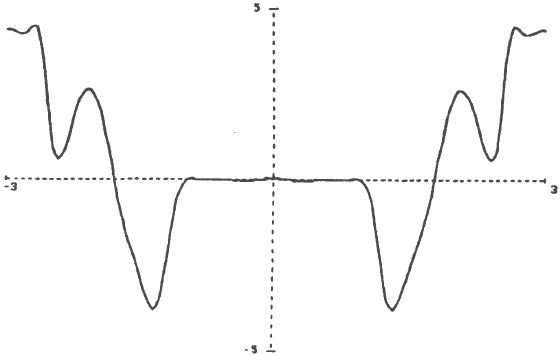
\includegraphics[scale=0.6]{PERFUNC Error Graph}
\caption{Values of the error of the output signals of a network trained to represent the sine function $g_2(x)$ at five grid points, drawn as a function of the frequency parameter $c_1$. Outside the region used for training, $-1<c_1<+1$, the error rapidly increases.}\label{PERFUNCErrorGraph}
\end{figure}

Experience with the back-propagation algorithm shows that learning becomes very slow when many hidden layers of some complexity are involved. To train networks with a large number of hidden layers the use of alternative strategies, such as the genetic algorithms seems to be advantageous.
%x_i x_i' should be distinguished in the index
\subsection{Snapshots}
\begin{figure}[h!t]
\centering
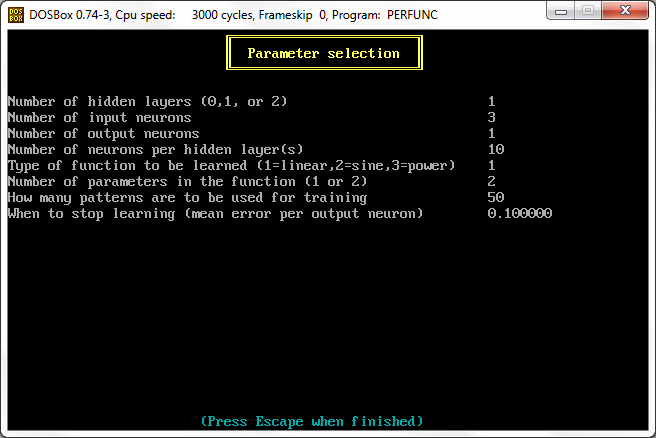
\includegraphics[scale=0.55]{PERFUNC_Capture_1}
\caption{Selection of the network architecture and parameters.}\label{PERFUNC_Capture_1}
\end{figure}
\begin{figure}[h!t]
\centering
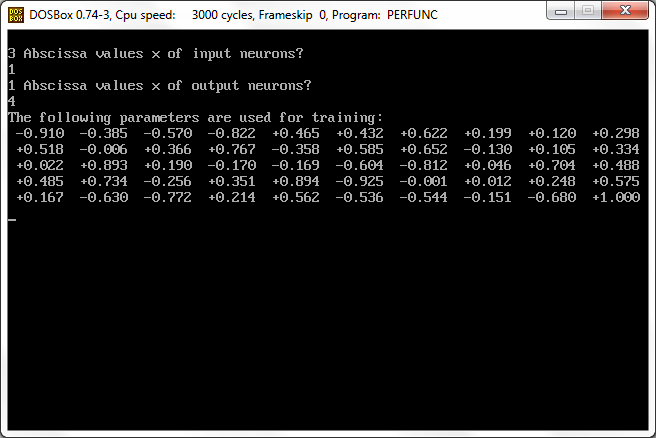
\includegraphics[scale=0.55]{PERFUNC_Capture_2}
\caption{Insertion of the learning dataset ($x_i=1,3,5$, $x_i'=4$).}\label{PERFUNC_Capture_2}
\end{figure}
\begin{figure}[h!t]
\centering
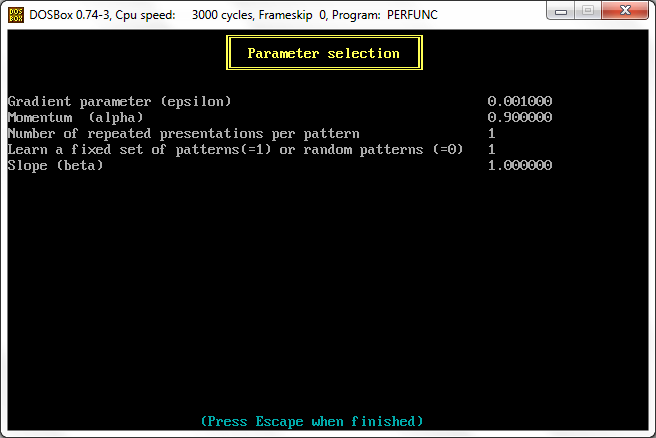
\includegraphics[scale=0.55]{PERFUNC_Capture_3}
\caption{Parameters of the learning protocol.}\label{PERFUNC_Capture_3}
\end{figure}
\begin{figure}[h!t]
\centering
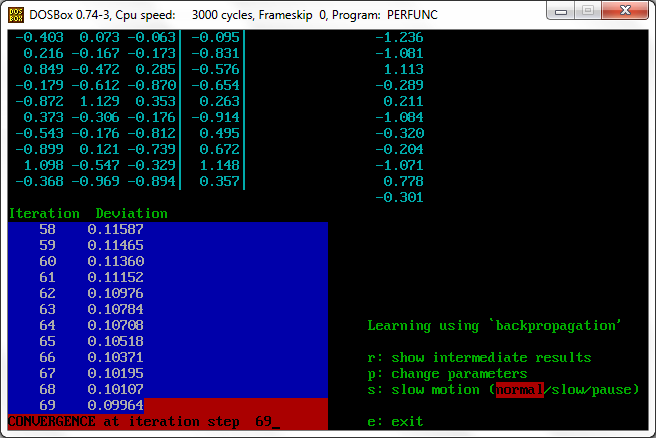
\includegraphics[scale=0.55]{PERFUNC_Capture_4}
\caption{Display of the training iterations.}\label{PERFUNC_Capture_4}
\end{figure}
\begin{figure}[h!t]
\centering
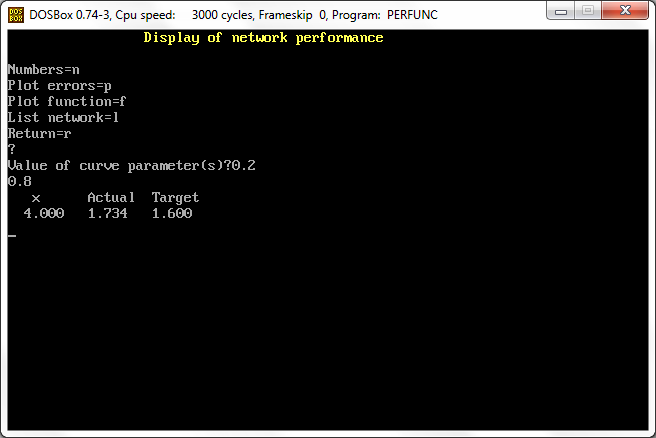
\includegraphics[scale=0.55]{PERFUNC_Capture_5}
\caption{Network performance.}\label{PERFUNC_Capture_5}
\end{figure}
\begin{figure}[h!t]
\centering
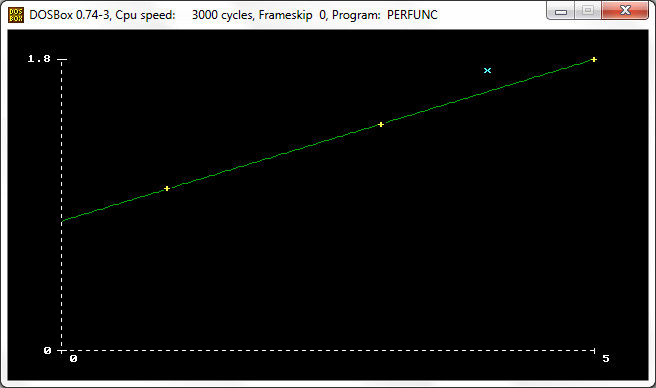
\includegraphics[scale=0.55]{PERFUNC_Capture_6}
\caption{Graphic representation ($c_1=0.2$, $c_2=0.8$).}\label{PERFUNC_Capture_6}
\end{figure}